\chapter{Neutron Yield Analysis}\label{chap:results}

%\section{Methodology}
%
%Ideally if one wants to measure the neutron yield by muons, one can shoot a monoenergetic muon beam at an infinite-long target and surround the target with a $4\pi$ detector which are able to identify and measure the momentum of all generated particles. This kind of idealization can be achieved closely with Daya Bay experiment.
%
%\begin{figure}
%\centering
%\begin{tikzpicture}
%	\draw (0,0) ellipse (.1cm and .2cm);
%	\draw (0,0) ellipse (1cm and 2cm);
%	\draw (0,.2) -- (3,.2);
%	\draw (0,-.2) -- (3,-.2);
%\end{tikzpicture}
%\caption{An ideal muon induced neutron measurement} \label{fig:IdealMuN}
%\end{figure}
%
%Suppose we know the muon track with some reconstruction algorithm. For those muons passing through the inner acrylic vessel(IAV), we can form a imaginary cylinder coaxial with the track which is fully contained in the IAV. If we fix the radius of the imaginary cylinder, for each track we have to adjust its length so as to make the cylinder fully contained in the IAV. Only neutrons captured in the imaginary cylinder count. If we concatenate the imaginary cylinders one after another, the ideal experiment is approximately realized, with some differences,
%\begin{enumerate}
%	\item Underground muons are not monoenergetic.
%	\item The imaginary cylinders serve as both the target and the detector.
%	\item Generated particles are hard to detect except neutrons.
%\end{enumerate}
%
%Although most underground experiments are not designed for measuring the neutron yield by muons, a in situ measurement of neutron background is still desirable. Since the energy of the underground muons can never be controlled, instead of measuring neutron yield as a function of the incident muon energy, a common practice is to measure neutron yield as a function of the incident \emph{mean} muon energy. And since this measurement is \emph{inclusive}, we don't have to know every detail of each intermediate particle leading to neutron production.

\section{Methodology}
%We propose a track-by-track geometric method to account for the neutron spill-in/spill-out effects which can be compared with a full neutron Monte Carlo simulation once it is available.
We measured the neutron yield on a track-by-track basis by choosing a well-defined fiducial volume for the produced neutrons, and corrected for inefficiencies by simple Monte Carlo simulations.

Neutron yield is the number of neutrons produced by a muon when it traverses a unit length of the material. In this study we are interested in the neutrons produced in the target material, GdLS. The GdLS not only serves as the target, but also serves as the neutron detector. Once a produced neutron is captured on Gd, the neutron position can be reconstructed with a 20 cm resolution~\cite{docdb7334}. In Daya Bay's experimental halls, muons come at all angles and penetrate the inner acrylic vessel (IAV) from all points and angles. Assuming the neutron capture position is axially symmetric around the muon track, a cylindrical fiducial volume can be constructed around the track fully enclosed in the GdLS. We consider the spill-in/spill-out corrections for the longitudinal and lateral directions separately.

\begin{figure}[ht]
	\centering
	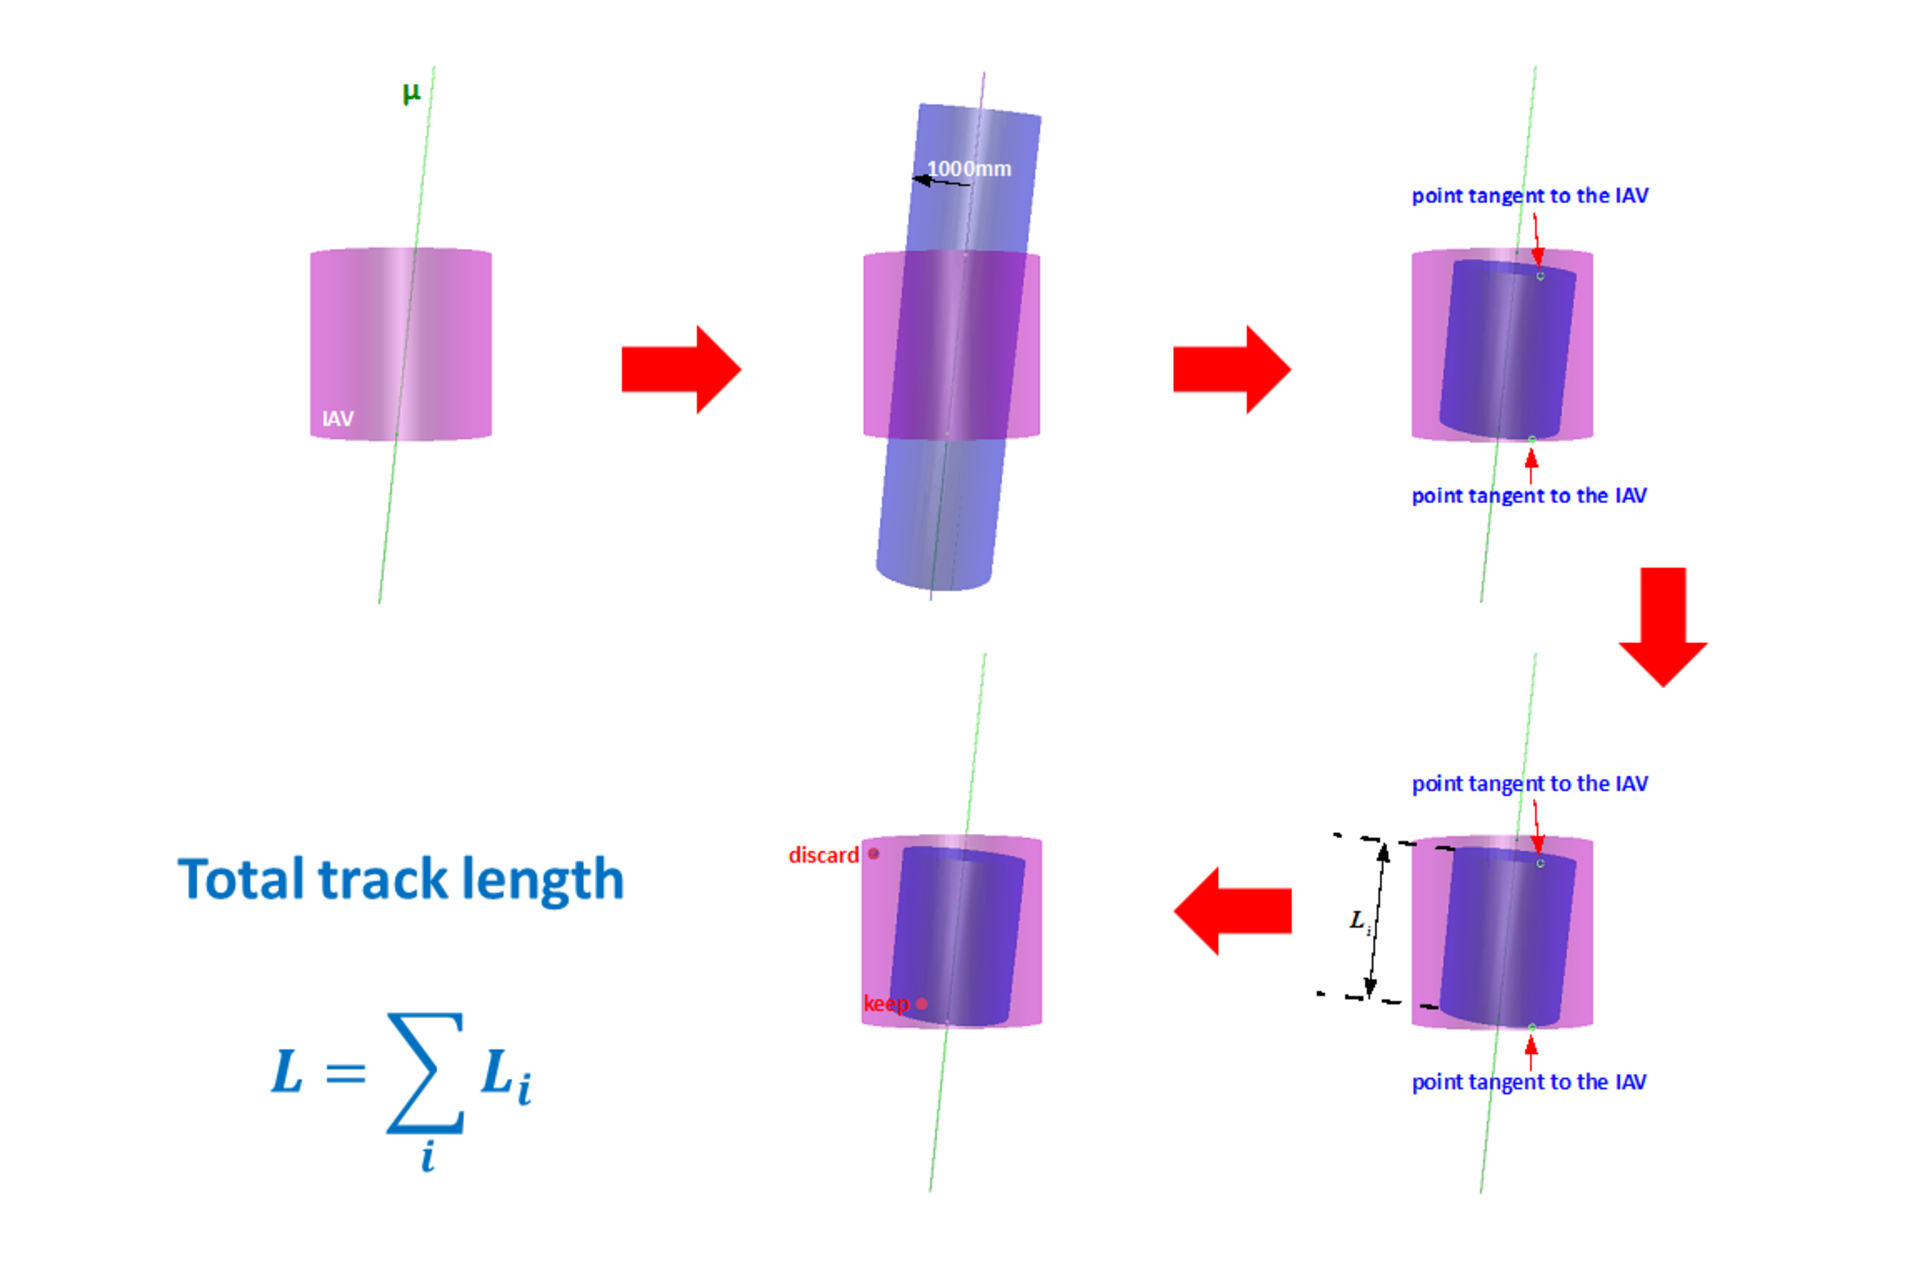
\includegraphics[width=\textwidth]{figures/chap7/fiducial_illustration.eps}
	\caption{A cartoon showing how a symmetric fiducial volume is constructed.}
	\label{fig:fiducial_illustration}
\end{figure}

A longest cylinder of one meter radius is inscribed in the IAV. Figure~\ref{fig:fiducial_illustration} shows how a symmetric fiducial volume can be constructed given a reconstructed muon track. The details of the construction is described in Appendix~\ref{app:a}.
After constructing the fiducial volume, the height of the inscribed fiducial cylinder is taken as the muon track length. Only neutrons captured within the fiducial cylinder are kept.


\section{Event Selection}

\subsection{Muon Selection}

Since a muon can traverse multiple detectors at a time, a muon is actually identified as a group of muon triggers across detectors in data.

The muon selection starts with muon triggers grouped in the directory \scriptsize\path{/Event/Data/Physics/Spallation} \normalsize in production files. The grouping first identifies whether a trigger satisfies the MuonAny criteria. MuonAny is the loosest muon tag which includes all triggers with IWS NHIT $>$ 6 or OWS NHIT $>$ 8 or AD charge $>$ 3000 pe or RPC 3/4 or 4/4 layers being fired (i.e., excluding the RPC random triggers). All MuonAny triggers have to be within 300 ns after the first MuonAny trigger in order to form the so called MuonPrompt triggers which completes the muon grouping process. For more details, see Ref.~\cite{docdb6759} . In order to reconstruct a muon track, a valid OWS reconstructed point with PoolSinple algorithm and a valid RPC reconstructed point with RpcSimple algorithm are required. Note that requiring a valid RPC point will rule out RPC random triggers automatically. Finally, in order to apply the fiducial cut, only tracks around which a fiducial cylinder with radius 1000 mm can fit in the IAV are kept.

\vspace{\baselineskip}
To summarize the muon selection criteria, a muon track has to
\begin{itemize}
  \item satisfy MuonAny criteria:
        \\IWS NHIT $>$ 6 or OWS NHIT $>$ 8 or AD charge $>$ 3000 pe or RPC 3/4 trigger,
  \item all MuonAny triggers within 300 ns since the first MuonAny trigger,
  \item valid points with PoolSinple and RpcSimple so that a track is formed by two point connection, and
  \item tracks around which a cylinder with 1000 mm can fit in the IAV.
\end{itemize}

\subsection{Neutron Selection}\label{sec:n_select}

The neutron has to be Gd captured within the fiducial volume. A Gd captured neutron is identified with its energy and timing. Here we use the IBD neutron energy cut, 6 MeV $< E_n <$ 12 MeV. For the timing cut we first choose the upper bound at 1000 $\mu$s after the muon, which could be fine tuned and optimized. The lower bound is set at 20 $\mu$s after the muon to avoid PMT ringing and AD retriggers. Also the flasher cut is applied to ensure the event is physical.

\vspace{\baselineskip}
To summarize the neutron selection criteria, the neutron has to satisfy the following:
\begin{itemize}
  \item 6 MeV $<$ $E_n$ $<$ 12 MeV,
  \item 20 $\mu$s $<$ $t_n-t_\mu$ $<$ 1000 $\mu$s,
  \item within the fiducial volume constructed in muon selection, and
  \item non-flasher event.
\end{itemize}


\section{Neutron Yield}
Measuring the neutron yield is closely related to measuring the muon-nucleus total interaction cross section since the number of neutrons produced can be written as
\begin{equation} \label{eq:neutron_number}
	\bar{N}_n=n\left\langle\nu\sigma\right\rangle\ell=\frac{\rho N_A}{A}\left\langle\nu\sigma\right\rangle\ell
\end{equation}
where $\bar{N}_n$ is the mean number of neutrons produced per muon, $n$ is the number density of the medium nuclei the muon traverses, $\nu$ is the neutron multiplicity per interaction, $\sigma$ is the inclusive neutron production cross section, $\ell$ is the mean track length of the muon, $\rho$ is the mass density of the medium, $N_A$ is the Avogadro number, and $A$ is the atomic mass of the medium. Because muons could interact with different nuclei in the medium and produce different number of neutrons, the mean value of the product $\left\langle\nu\sigma\right\rangle$ is used.

Experimentally, the neutron yield is given by
\begin{equation} \label{eq:ideal_neutron_yield}
	Y_n=\frac{\bar{N}_n}{\ell\rho}=\frac{N_n}{L\rho}
\end{equation}
where $Y_n$ is the neutron yield, $N_n$ is the total number of neutrons produced by all selected muons and $L$ is the total muon track length traversed by all selected muons.

From Eqs.~\ref{eq:neutron_number} and ~\ref{eq:ideal_neutron_yield} the mean value of the product of the neutron multiplicity and the muon-nucleus total interaction cross section is
\begin{equation}
	\left\langle\nu\sigma\right\rangle=\frac{Y_nA}{N_A}
\end{equation}

However, since 100\% neutron detection efficiency cannot be achieved experimentally due to the neutron selection cuts and finite detector acceptance, the produced number of neutrons is determined by $N_n^s/\epsilon$, the number of observed neutrons corrected by the total detection efficiency which is a product of several efficiency terms. In this study, the total detection efficiency
\begin{equation}
	\epsilon=\epsilon_{Gd}\epsilon_E\epsilon_T\epsilon_{acc}
\end{equation}
where $\epsilon_{Gd}$ is the Gd capture ratio, $\epsilon_E$ is the energy cut efficiency, $\epsilon_T$ is the timing cut efficiency and $\epsilon_{acc}$ is the detector acceptance due to the fiducial volume cut.

The yield formula used in this study is hence
\begin{equation}
	Y_n=\frac{N_n^s}{\epsilon_{Gd}\epsilon_E\epsilon_T\epsilon_{acc}L\rho}
\end{equation}

Since the muon-nucleus total interaction cross section depends on the muon energy, the neutron yield also does. It is standard to parametrize the energy dependence as a power law~\cite{Zatsepin1965},
\begin{equation}
	Y_n(\bar{E}_\mu)=\alpha\bar{E}_\mu^\beta
\end{equation}
where $\bar{E}_\mu$ is the mean muon energy and $\alpha$ and $\beta$ are parameters to be fitted with data. This formula is largely confirmed by FLUKA and GEANT4 simulations~\cite{Wang2001}~\cite{Araujo2005}~\cite{Mei2006}~\cite{Malgin2008} as well as by measurements~\cite{Bezrukov1973}~\cite{Enikeev1987}~\cite{Aglietta1989}. However large tensions in the values of $\alpha$ and $\beta$ still remain. The Daya Bay experiment has three experimental halls each with different overburden. Therefore, Daya Bay, a single experiment, can measure three yield values corresponding to three different mean muon energies.

There are therefore 8 terms to be determined in order to measure the yield as a function of the mean muon energy, namely $N_n^s$, $\epsilon_{Gd}$, $\epsilon_E$, $\epsilon_T$, $\epsilon_{acc}$, $L$, $\rho$, and $\bar{E}_\mu$. In the following sections each term and its uncertainty will be discussed in detail.

The discussion will start with more widely studied quantities and move on to the quantities more specific to this study.

\subsection{Target Density \texorpdfstring{$\rho$}{rho}}
The GdLS density is~\cite{docdb6615}
\begin{equation}
	\rho=0.861\pm 0.001\text{ }g/cm^3
\end{equation}

\subsection{Gd Capture Ratio \texorpdfstring{$\epsilon_{Gd}$}{epsilon Gd}}
Spallation neutrons generated in the target mass, GdLS, may not all be captured on Gd. Some could be captured on H or other nuclei. Some are not captured at all and leave the detector, which we call spill-out neutrons. There are also spill-in neutrons, namely neutrons generated outside and transported into the fiducial volume and get captured on Gd. Since in this study we select only the Gd captured neutrons, we have to determine this efficiency which is often called the Gd capture ratio.

Many studies had been done on the Gd capture ratio with spallation neutrons~\cite{docdb7273}~\cite{docdb7524}~\cite{docdb7525}, calibration sources~\cite{docdb7273}~\cite{docdb7525}, special calibration runs~\cite{docdb8280}~\cite{docdb8473}~\cite{docdb8501}~\cite{docdb9226}~\cite{docdb9273}, and Monte Carlo simulation~\cite{docdb7730}. However, different studies adopt slightly different definitions of this ratio. Here we define the Gd capture ratio as
\begin{equation} \label{eq:gd_capture_ratio}
	\epsilon_{Gd}=\frac{\text{number of neutrons generated in GdLS and captured on Gd}}{\text{number of neutrons generated in GdLS}}
\end{equation}

We use the more up-to-date study~\cite{docdb9273}. In this study a complete comparison between AmC, AmBe, PuC, and Monte Carlo is given and the efficiency due to energy cuts is corrected for resulting in a $\epsilon_{Gd}$ definition which coincides with Eq.~\ref{eq:gd_capture_ratio}. The final result is quoted as,
\begin{equation}
  \epsilon_{Gd}=85.2\%\pm 0.4\%
\end{equation}


\subsection{Energy Cut Efficiency \texorpdfstring{$\epsilon_{E}$}{epsilon E}}

One of the signatures of a neutron captured on Gd is the 8 MeV $\gamma$ energy released from the de-excitation of Gd*. Therefore, we use the 8 MeV energy cut efficiency published in the IBD analysis~\cite{dayabay2012_1}, combining the correlated and uncorrelated uncertainties,
\begin{equation}
	\epsilon_{E}=90.9\%\pm 0.61\%
\end{equation}


\subsection{Capture Time Cut Efficiency \texorpdfstring{$\epsilon_{T}$}{epsilon T}}

The other signature of a neutron captured on Gd is the capture time whose mean value is $\sim 28\mu s$. Figure~\ref{fig:IBD_capture_time} shows the IBD neutron capture time distribution. The distribution is not a simple exponential but has a rising edge in the beginning of the spectrum. A 2-exponential fit to model the whole spectrum~\cite{docdb7299}, one of which accounts for the rising edge due to the thermalization of neutrons.
\begin{figure}
	\centering
	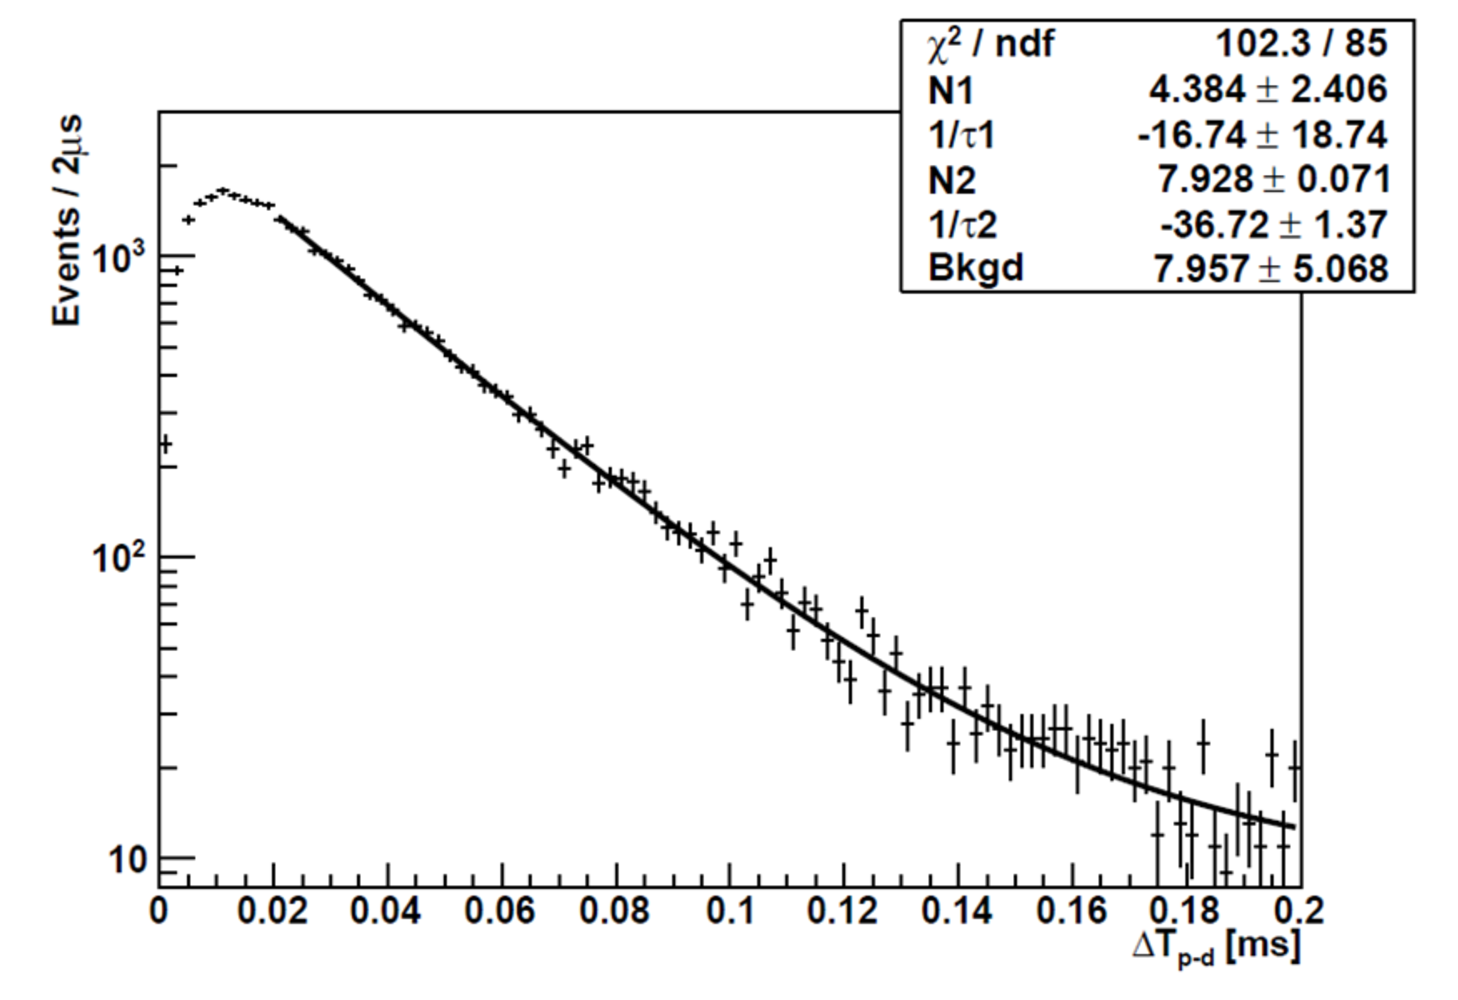
\includegraphics[width=.6\textwidth]{figures/chap7/IBD_capture_time.eps}
	\caption[IBD neutron capture time distribution]{IBD neutron capture time distribution~\cite{docdb7299}}
	\label{fig:IBD_capture_time}
\end{figure}

In the spallation neutron case, there are several differences. First, the initial energy of the spallation neutrons can be higher than the IBD neutrons, leading to a longer thermalization time. Second, after the muon passes through the AD, the huge amount of energy distorts the PMT signal for about 10 $\mu$s and produce retrigger events. Figure~\ref{fig:spallation_capture_time} shows the capture time distribution of EH1 AD1.
\begin{figure}[ht]
	\centering
	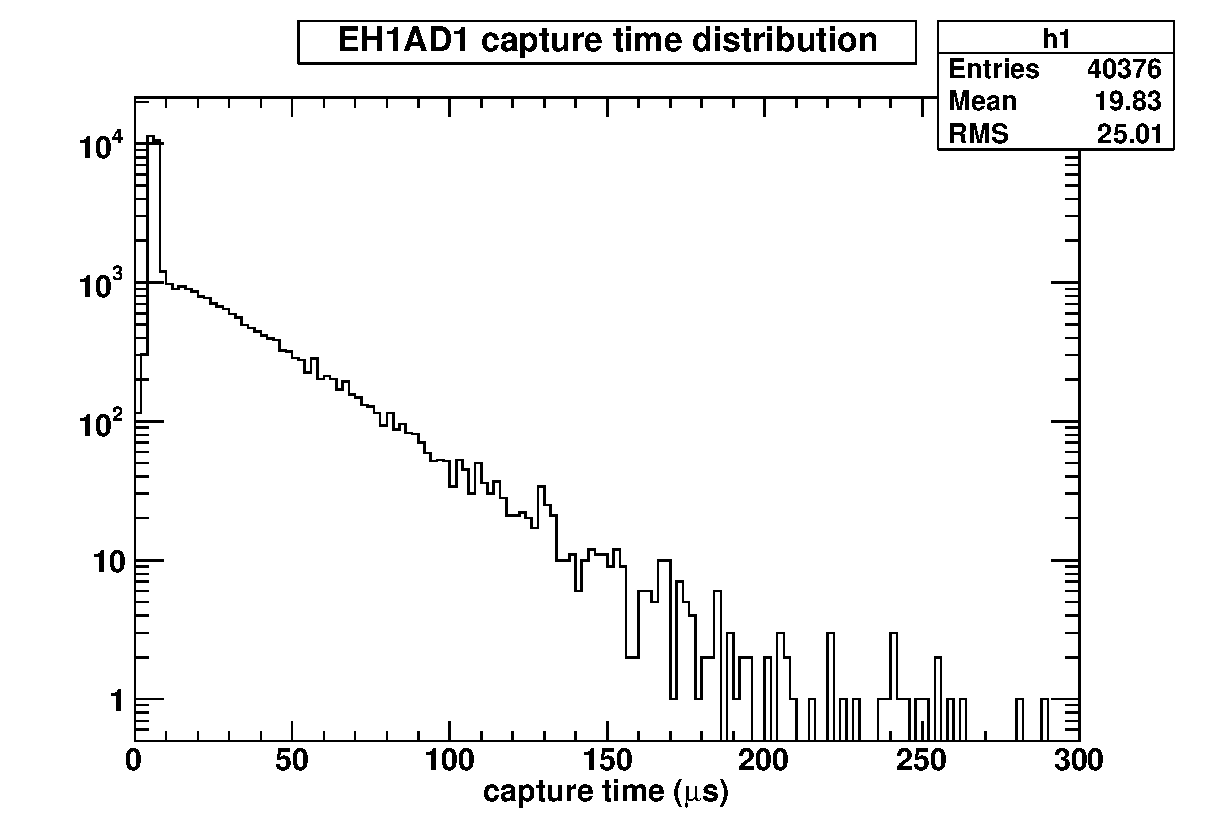
\includegraphics[width=.6\textwidth]{figures/chap7/spallation_neutron_capture_time.eps}
	\caption{Spallation neutron capture time distribution}
	\label{fig:spallation_capture_time}
\end{figure}
Clearly there is a retrigger peak between 4 and 10 $\mu$s. In the 2-exponential function model, we can do a linear interpolation between the time with the left and right bins. Then we fit the distribution to a 2-exponential function, and use the fitted function to estimate the capture time cut efficiency. Figure~\ref{fig:fit_capture_time} shows the fit result of EH1 AD1.
\begin{figure}[ht]
	\centering
	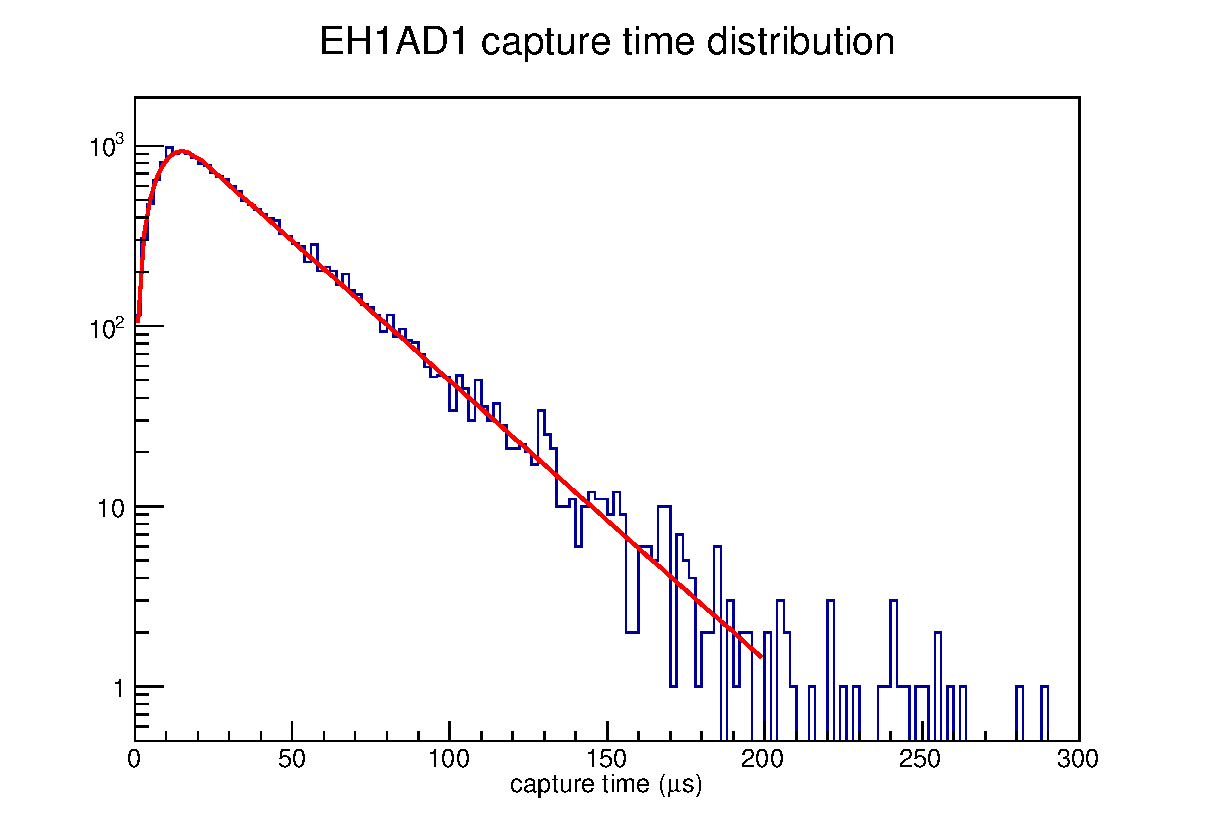
\includegraphics[width=.6\textwidth]{figures/chap7/fit_capture_time.eps}
	\caption{2-exponential fit to the interpolated capture time distribution}
	\label{fig:fit_capture_time}
\end{figure}
The efficiency is then obtained by the formula
\begin{equation}
	\epsilon_T=\frac{\int_{20}^{\infty}f(t)dt}{\int_{0}^{\infty}f(t)dt}
\end{equation}
The systematic uncertainty of this number is obtained by varying the counts in the 4 to 10 $\mu$s window, fitting the distribution with the 2-exponential function, and calculating the efficiency with the new fitted function. A $5\%$ relative uncertainty is found for all ADs. The results of capture time cut efficiency are summarized in Table~\ref{tab:timing_efficiency}.
\begin{table}[ht]
	\centering
	\begin{tabular}{|c|c|}
		\hline
		detector & $\epsilon_T$ (\%) \\
		\hline
		EH1 AD1 & 0.64$\pm$0.03 \\
		\hline
		EH1 AD2 & 0.64$\pm$0.03 \\
		\hline
		EH2 AD1 & 0.63$\pm$0.03 \\
		\hline
		EH3 AD1 & 0.66$\pm$0.03 \\
		\hline
		EH3 AD2 & 0.66$\pm$0.03 \\
		\hline
		EH3 AD3 & 0.67$\pm$0.03 \\
		\hline
	\end{tabular}
	\caption{Capture time cut efficiency for each AD.}
	\label{tab:timing_efficiency}
\end{table}


\subsection{Number of Selected Neutrons \texorpdfstring{$N_n^s$}{N} and Total Track Length \texorpdfstring{$L$}{L}}
There are uncertainties in the vertex in the RPC and OWS reconstruction. Thus, the RPC-OWS connection is also subject to these uncertainties and deviates from the true track, which in turn leads to a different fiducial cylinder from the real one. Not only the total track length, which is the sum of the heights of all fiducial cylinders, but also the number of neutrons included in the fiducial volume will change. So we discuss the number of selected neutrons together with the total track length, and estimate the uncertainties with a toy Monte Carlo which takes into account the geometry effects concerning the two numbers at the same time.

Neutron selection criteria were stated in Section~\ref{sec:n_select}. A side band time window between [1020, 2000] $\mu$s is used for the background spectrum. Figure~\ref{fig:energy_spectrum} shows the results for each AD.
\begin{figure}[ht]
	\centering
	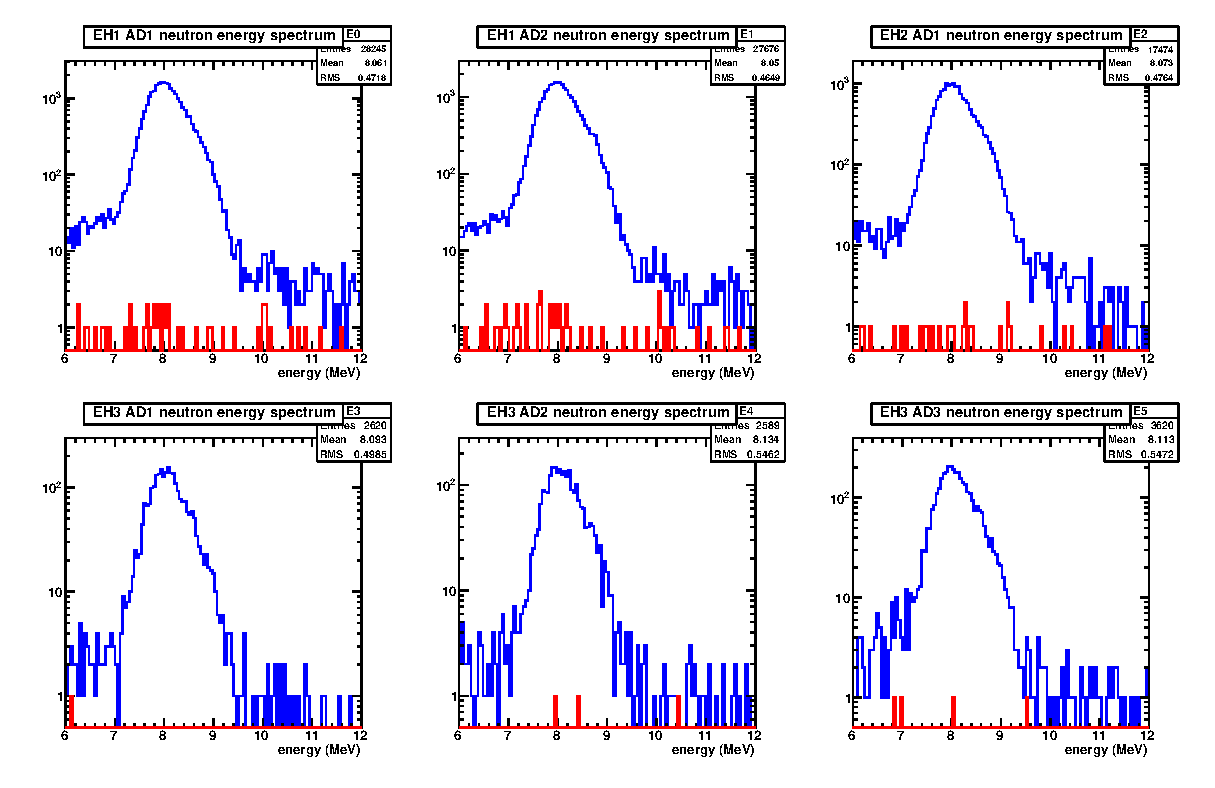
\includegraphics[width=\textwidth]{figures/chap7/neutron_energy_spectrum.eps}
	\caption{Neutron and background energy spectrum.}
	\label{fig:energy_spectrum}
\end{figure}
The number of selected neutron is $N_n^s=N_{sig}-N_{bkg}$, where $N_{sig}$ and $N_{bkg}$ are the numbers of events in the signal and the background windows, respectively. The statistical uncertainty is computed according to $\sqrt{N_{sig}+N_{bkg}}$. Table~\ref{tab:number_of_neutrons} lists the results for $N_{sig}$ and $N_{bkg}$.
\begin{table}[ht]
	\centering
	\begin{tabular}{|c|c|c|}
		\hline
		detector & $N_{sig}$ & $N_{bkg}$ \\
		\hline
		EH1 AD1 & 28245 & 44 \\
		\hline
		EH1 AD2 & 27676 & 51 \\
		\hline
		EH2 AD1 & 17474 & 28 \\
		\hline
		EH3 AD1 & 2620 & 1 \\
		\hline
		EH3 AD2 & 2589 & 3 \\
		\hline
		EH3 AD3 & 3620 & 4 \\
		\hline
	\end{tabular}
	\caption{Results of events in the signal and the background windows.}
	\label{tab:number_of_neutrons}
\end{table}

The total track length is obtained by summing the lengths of the fiducial cylinders. The results are listed in Table~\ref{tab:total_track_length}.
\begin{table}[ht]
	\centering
	\begin{tabular}{|c|c|}
		\hline
		detector & total track length (cm) \\
		\hline
		EH1 AD1 & $1.17\times 10^9$ \\
		\hline
		EH1 AD2 & $1.13\times 10^9$ \\
		\hline
		EH2 AD1 & $6.90\times 10^8$ \\
		\hline
		EH3 AD1 & $7.78\times 10^7$ \\
		\hline
		EH3 AD2 & $7.26\times 10^7$ \\
		\hline
		EH3 AD3 & $9.69\times 10^7$ \\
		\hline
	\end{tabular}
	\caption{Total track length for each AD.}
	\label{tab:total_track_length}
\end{table}

The systematic uncertainties for $N_n^s$ and $L$ are estimated by a toy Monte Carlo which takes into account the uncertainties due to the vertex reconstructions. A deviation in track will change the construction of the fiducial cylinder, which might in turn change the inclusion or exclusion of a neutron. Therefore this toy Monte Carlo will estimate the two systematic uncertainties at the same time. The procedure of the toy Monte Carlo is:
\begin{itemize}
	\item Take the small muon Monte Carlo sample.
	\item Without loss of generality, take the RPC and OWS reconstructed vertices as true vertices.
	\item Generate a true neutron vertex according to a uniform distribution along the track direction and a lateral distance according to the 2D gaussian function $re^{-\frac{r^2}{2\sigma^2}}$ where $\sigma=$ 40 cm. From data we know when $r$ is small this is a good approximation and 40 cm is obtained from data. The vertex could be anywhere in the IAV in order to study the inclusion/exclusion of neutrons due to the uncertainties in RPC, OWS and neutron vertices.
	\item Randomly select a point within the 25 cm $\times$ 25 cm square due to RPC resolution.
	\item Randomly generate a point around the OWS vertex with a random direction and a radial distance following the 3D gaussian function $r^2e^{-\frac{r^2}{2\sigma^2}}$, where $\sigma=$ 50 cm.
	\item Randomly generate a point around the neutron vertex with a random direction and a radial distance following the 3D gaussian function $r^2e^{-\frac{r^2}{2\sigma^2}}$, where $\sigma=$ 20 cm by Yasu's AdSimple resolution.
	\item Form the ``smeared'' track and construct the fiducial volume.
	\item For each neutron, record its selection status before and after the smearing process.
	\item For the true and smeared case, sum up the fiducial cylinder lengths and the number of neutrons in the fiducial cylinder.
\end{itemize}
The results show a $1\%$ uncertainty in the total track length and a $10\%$ uncertainty in the number of selected neutrons. Since the total uncertainty is dominated by the neutron selection uncertainty, the full covariance matrix is not calculated\footnote{
For a two variable differentiable function $f(a,b)$ the uncertainty in $f$ is
\begin{equation}
	\left(\frac{\sigma_f}{f}\right)^2\approx\left(\frac{\sigma_a}{a}\right)^2+\left(\frac{\sigma_b}{b}\right)^2+2\left(\frac{\sigma_a}{a}\right)\left(\frac{\sigma_b}{b}\right)\rho_{ab}
\end{equation}
where $\sigma_f$, $\sigma_a$, and $\sigma_b$ are uncertainties in $f$, $a$, and $b$, respectively, and $\rho_{ab}$ is the correlation coefficient of $a$ and $b$. Since $-1 \leq \rho_{ab} \leq 1$, if $\frac{\sigma_a}{a}\gg\frac{\sigma_b}{b}$, $\frac{\sigma_f}{f}\approx\frac{\sigma_a}{a}$.
}.


\subsection{Lateral Acceptance \texorpdfstring{$\epsilon_{acc}$}{epsilon}}
The neutrons are expected to be boosted forward. There is space before the fiducial cylinder. If neutrons are produced upstream, they enter the cylinder even if they are not produced inside. As a result, the neutron flux entering the fiducial cylinder from upstream of the track equals the neutron flux leaving the fiducial cylinder. We only need the lateral distribution to determine the detector acceptance. Figure~\ref{fig:z_distribution} shows the distribution of the relative longitudinal position of the capture point relative to the cylinder center. It clearly shows a uniform distribution, which shows spill-in equals spill-out in the longitudinal direction.
\begin{figure}[ht]
	\centering
	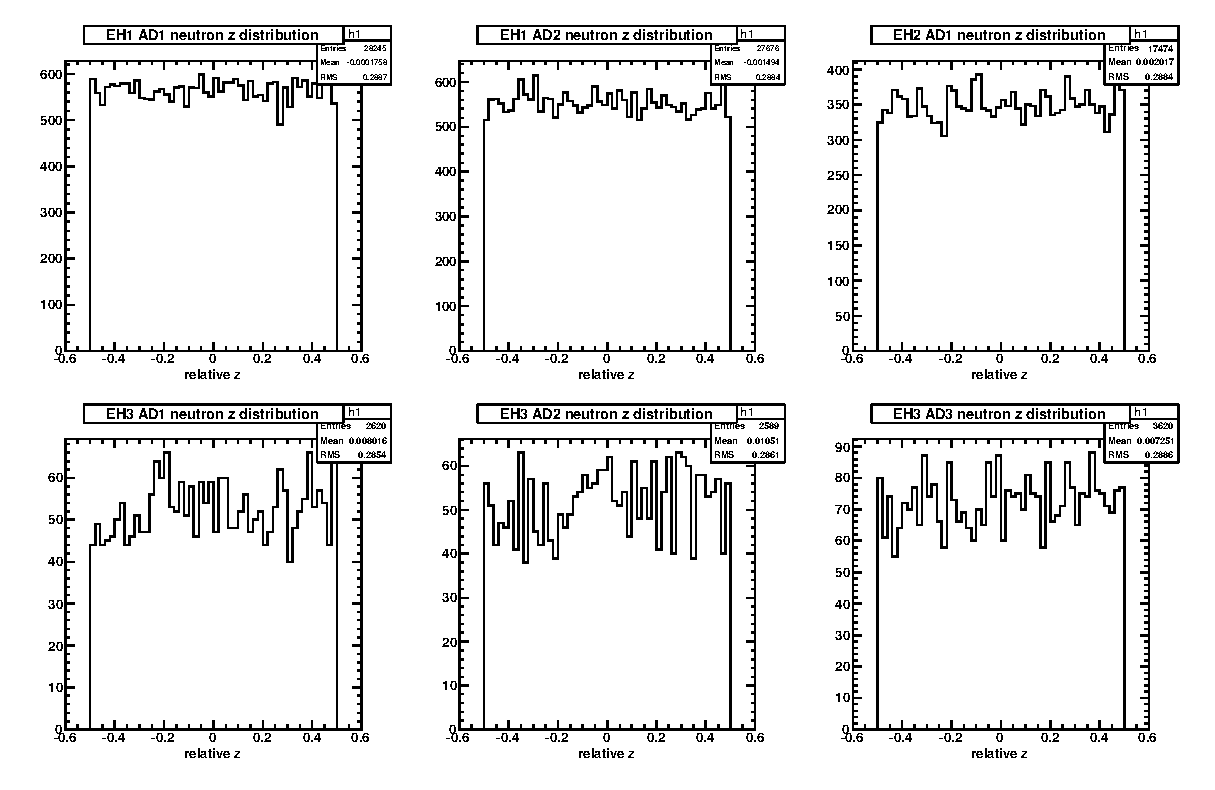
\includegraphics[width=\textwidth]{figures/chap7/z_distribution.eps}
	\caption{Relative longitudinal capture position with respect to the fiducial cylinder center.}
	\label{fig:z_distribution}
\end{figure}

To estimate the lateral acceptance due to the finite volume of the fiducial cylinders, we lift the muon selection criteria that a fiducial cylinder is able to be constructed. This mean we practically use every muons which have a track reconstructible by RPC-OWS connection. After the track reconstruction, we search for Gd captured neutrons and register the lateral distances to the track. Figure~\ref{fig:lateral_distance_no_cylinder} shows the lateral distance distribution for each AD.
\begin{figure}[ht]
	\centering
	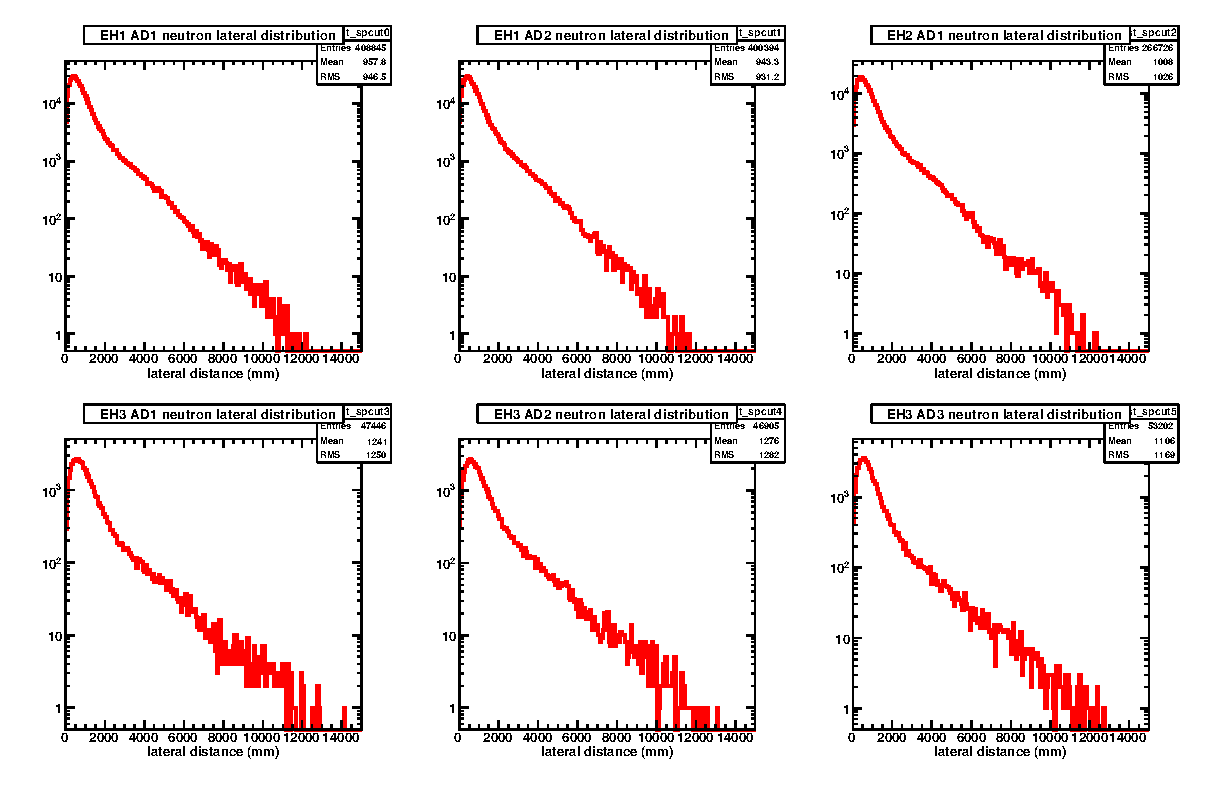
\includegraphics[width=\textwidth]{figures/chap7/lateral_distance_no_cylinder.eps}
	\caption{Neutron lateral distribution for muons with a valid RPC-OWS track.}
	\label{fig:lateral_distance_no_cylinder}
\end{figure}
Table~\ref{tab:lateral_acceptance} shows the lateral acceptance estimated by the fraction of the number of events with lateral distances smaller than 1000 mm.
\begin{table}
	\centering
	\begin{tabular}{|c|c|}
		\hline
		detector & lateral acceptance ($\%$) \\
		\hline
		EH1 AD1 & $0.60\pm 0.06$ \\
		\hline
		EH1 AD2 & $0.60\pm 0.06$ \\
		\hline
		EH2 AD1 & $0.61\pm 0.06$ \\
		\hline
		EH3 AD1 & $0.57\pm 0.06$ \\
		\hline
		EH3 AD2 & $0.56\pm 0.06$ \\
		\hline
		EH3 AD3 & $0.64\pm 0.06$ \\
		\hline
	\end{tabular}
	\caption{Lateral acceptance estimated by the method described in the text.}
	\label{tab:lateral_acceptance}
\end{table}


\subsection{Mean Muon Energy \texorpdfstring{$\bar{E}_\mu$}{E}}
Daya Bay cannot measure muon energy; Daya Bay only measures muon \emph{deposited} energy. Therefore, the mean muon energy is obtained by Monte Carlo simulation. A sample of muons for each hall was generated by the MUSIC package which has been incorporated in NuWa. Each MUSIC sample file contains a million muons with energies, angles (polar and azimuthal) on the sea level and energies and angles in the hall after propagation through the rocks. Therefore, for each hall a simulated mean muon energy can be obtained by simply taking the arithmetic mean of the muon energies after propagation. Figure~\ref{fig:muon_energy_spectrum} shows the simulated muon energy spectra \emph{in} the three halls. From these spectra we see that the more overburden a hall has, the harder (i.e., higher energy) the muon energy spectrum is. The mean muon energy for each hall is listed in Table~\ref{table:mean_muon_energy}.
\begin{figure}
	\centering
	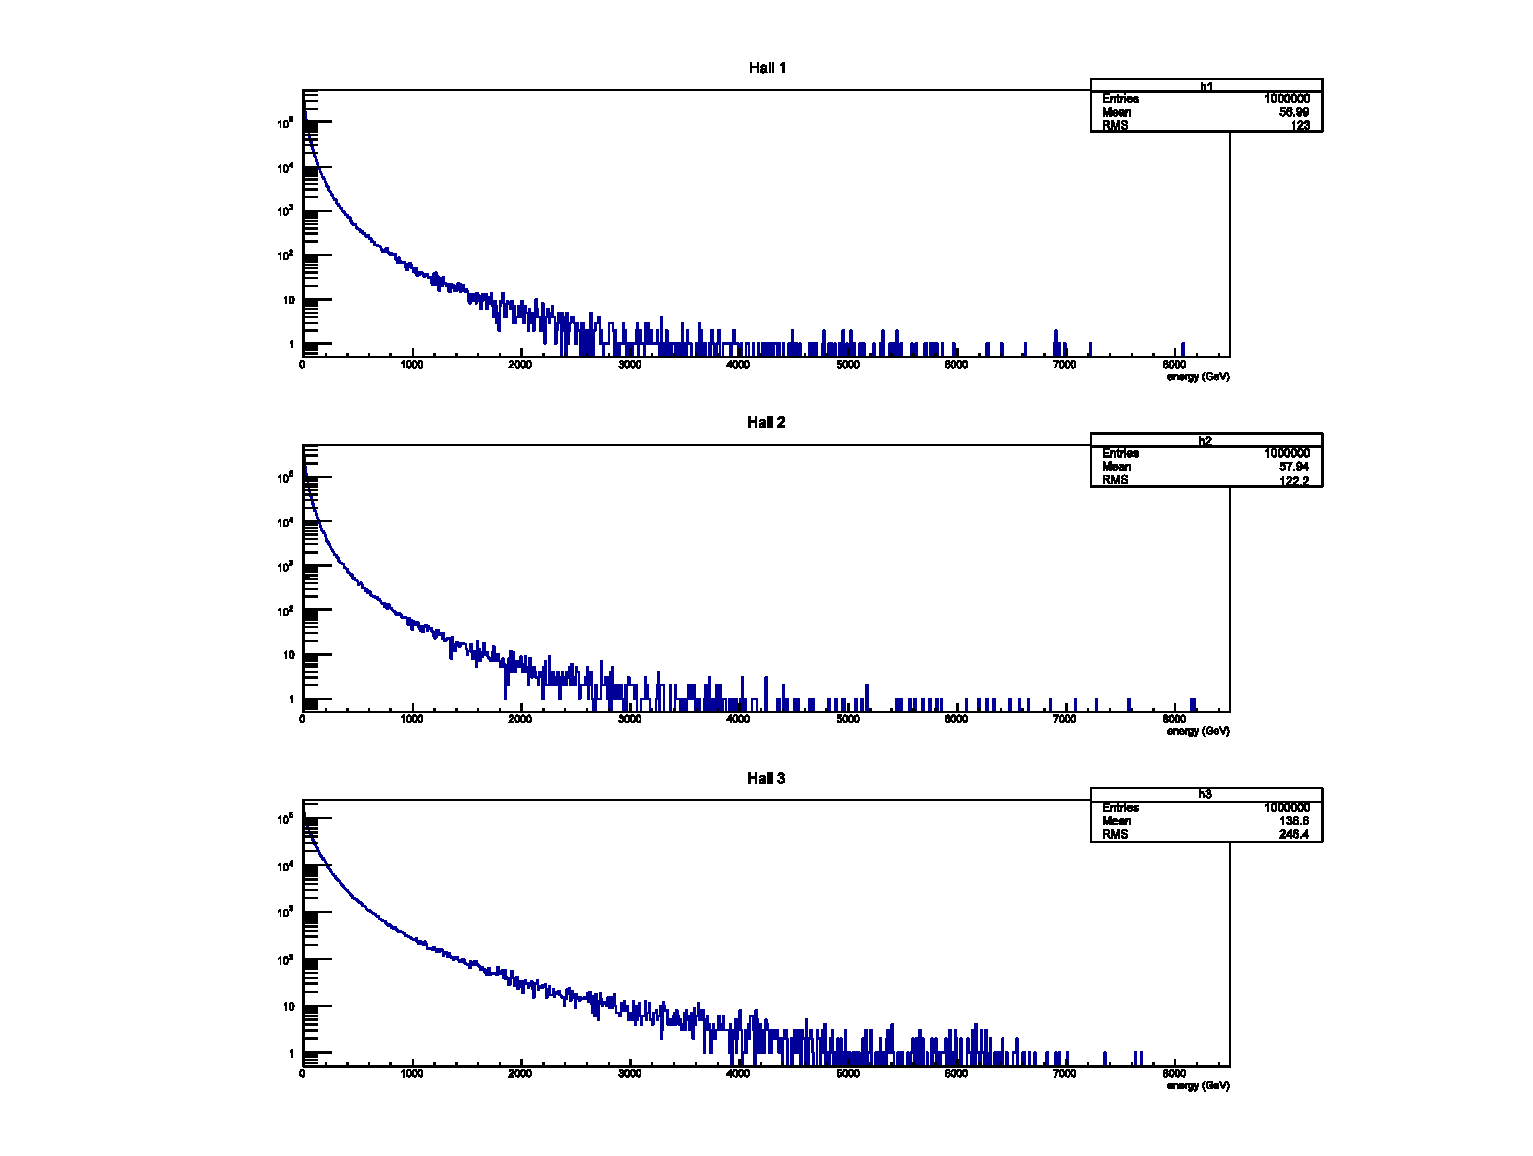
\includegraphics[width=\textwidth]{figures/chap7/muon_energy_spectrum.eps}
	\caption{Simulated muon energy spectra in the three halls.}
	\label{fig:muon_energy_spectrum}
\end{figure}
\begin{table}
	\centering
	\begin{tabular}{cccc}
	\toprule
	& EH1 & EH2 & EH3 \\
	\midrule
	mean muon energy (GeV) & 57 & 58 & 137 \\
	\bottomrule
	\end{tabular}
	\caption{The mean muon energy for each hall by simulation.}
	\label{table:mean_muon_energy}
\end{table}

However, in this study, not all muons are selected. Recall that in the muon selection criteria, a RPC-OWS track has to be formed, which implies a RPC hit. Consequently for an AD, it doesn't see all muons coming from all angles. Instead, it sees muons which happen to go through the RPC, in effect excluding muons with very large polar angles. This "RPC coverage" effect varies from AD to AD. Figure~\ref{fig:rpc_coverage} shows the RPC coverage for each AD in the 3 halls. Take hall 1 as an example. AD1 has more RPC coverage in south east. Therefore AD1 will sample more large angle muons from south east. On the contrary, AD2 samples more large angle muons from north west. Since the mountain overburden is not uniform (see Figure~\ref{fig:muontain_profile}), and since muons incident from different direction go through different amount of rocks, the mean muon energy will not only be different from the hall average, but will have an AD-to-AD variation.
\begin{figure}
	\centering
	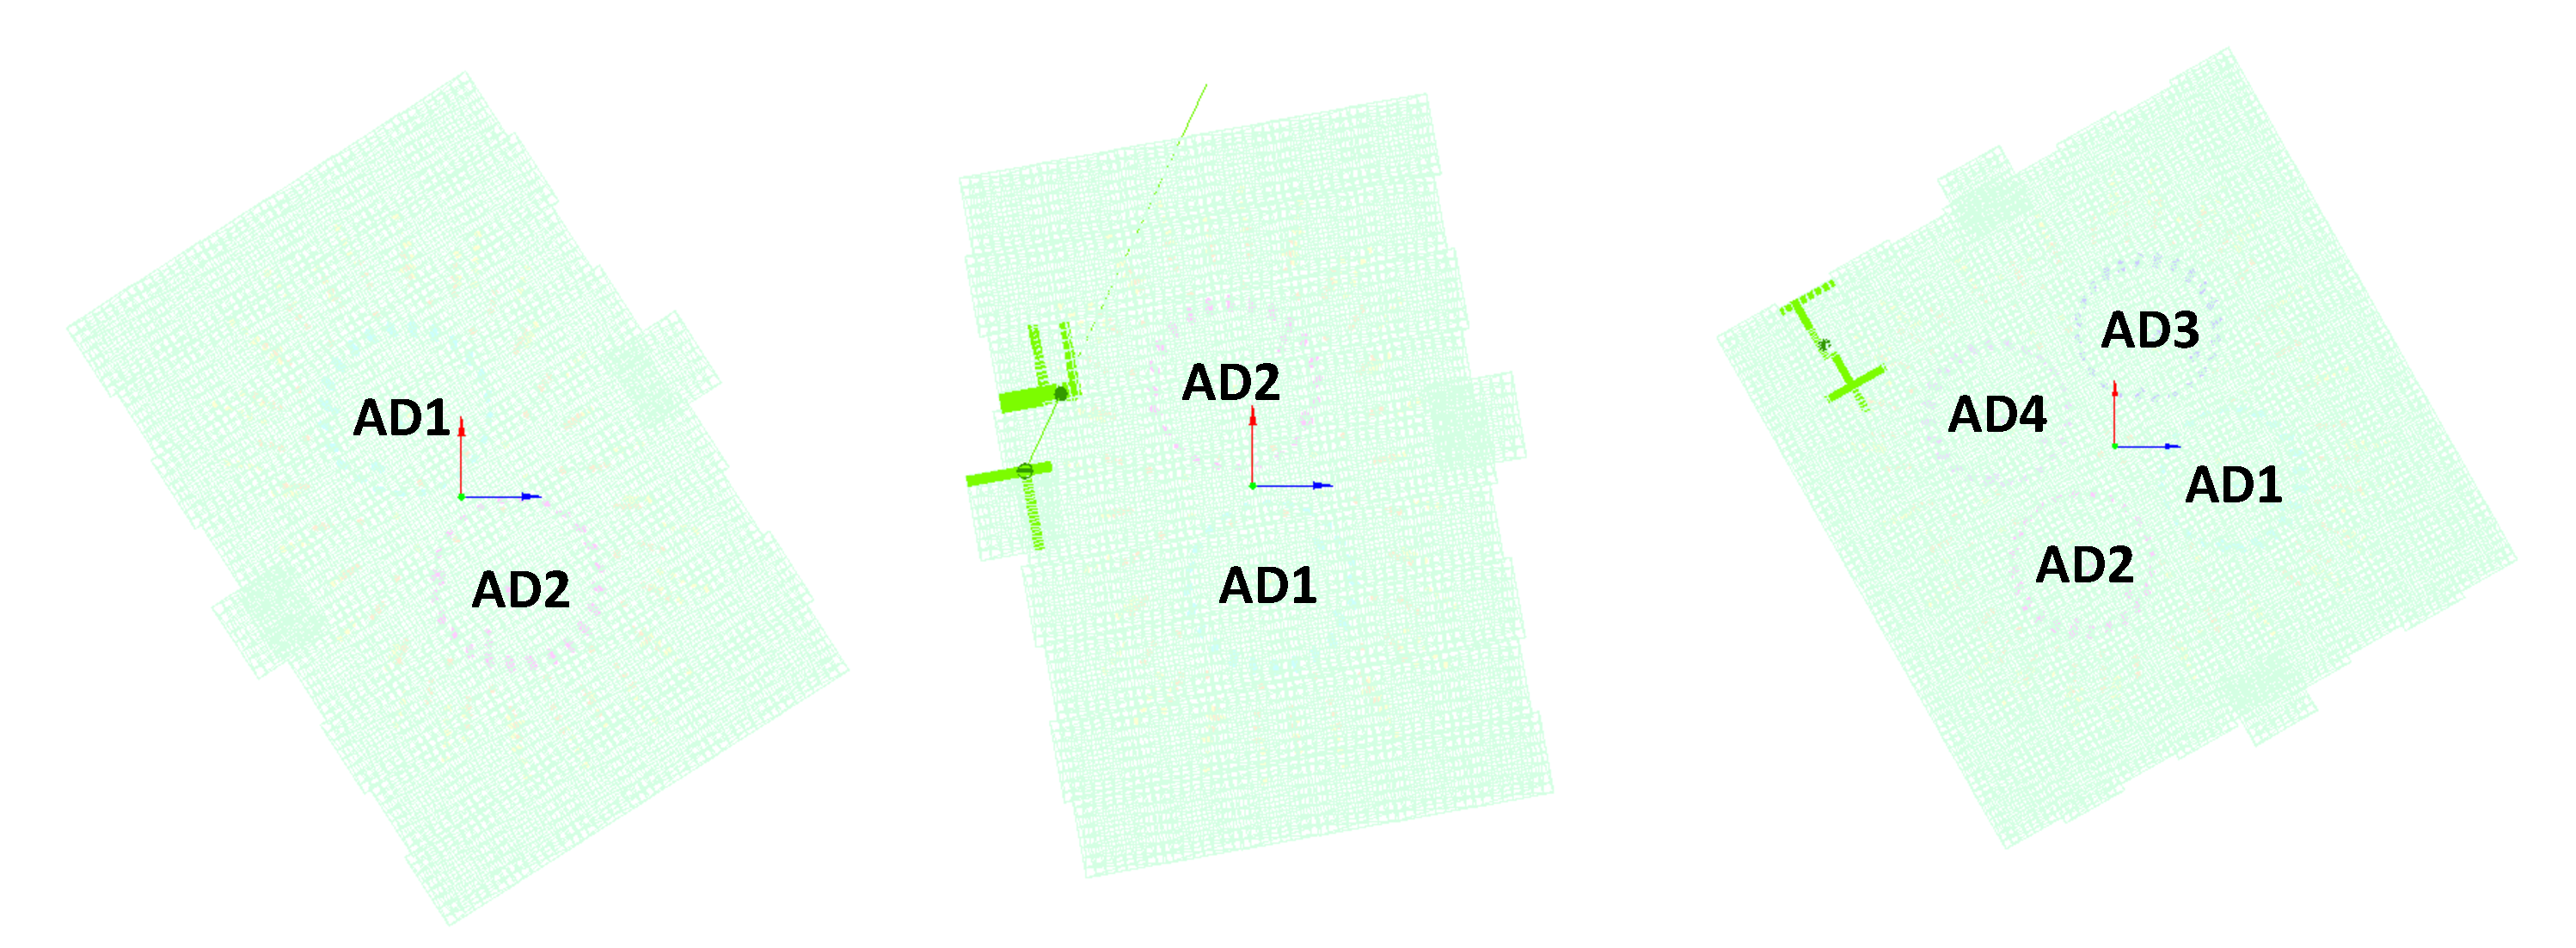
\includegraphics[width=\textwidth]{figures/chap7/RPC_coverage.eps}
	\caption{RPC coverage for each AD in different halls.}
	\label{fig:rpc_coverage}
\end{figure}
\begin{figure}
	\centering
	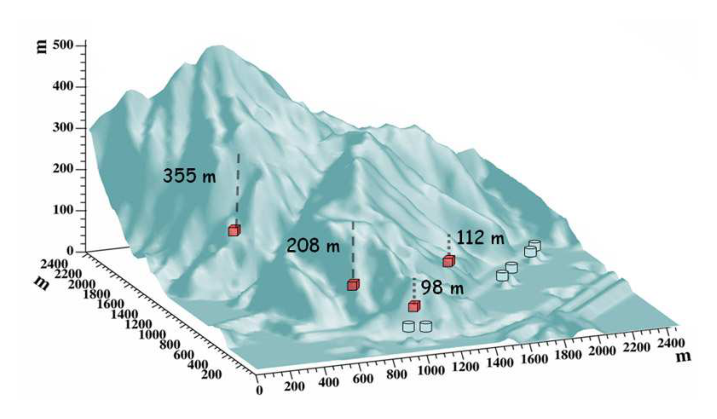
\includegraphics[width=0.7\textwidth]{figures/chap7/mountain_profile.eps}
	\caption[Three dimensional profile of Pai Ya Mountain, where the Daya Bay experimental halls are located including the water hall.]{Three dimensional profile of Pai Ya Mountain, where the Daya Bay experimental halls are located including the water hall.~\cite{dayabay_proposal}}
	\label{fig:muontain_profile}
\end{figure}

To account for the RPC coverage effect, a resampling of the MUSIC sample was done. The procedure of the resampling is:
\begin{itemize}
	\item In the RPC plane, generate a random point.
	\item Generate a direction according to the angular distribution in the MUSIC sample.
	\item Form the track. If for the track a fidicial cylinder can be constructed for a particular AD, keep it. Otherwise don't keep it.
	\item Repeat the procedure for all ADs.
\end{itemize}
The results of the resampling is shown in Table~\ref{tab:mean_muon_energy}. A $5\%$ systematic uncertainty due to the incomplete knowledge in the rock composition and the resolution in the mountain profile is assigned.
\begin{table}
	\centering
	\begin{tabular}{|c|c|}
		\hline
		detector & mean muon energy (GeV) \\
		\hline
		EH1 AD1 & $47\pm 2$ \\
		\hline
		EH1 AD2 & $47\pm 2$ \\
		\hline
		EH2 AD1 & $50\pm 2$ \\
		\hline
		EH3 AD1 & $123\pm 6$ \\
		\hline
		EH3 AD2 & $130\pm 7$ \\
		\hline
		EH3 AD3 & $127\pm 6$ \\
		\hline
	\end{tabular}
	\caption{Mean muon energy seen by each AD.}
	\label{tab:mean_muon_energy}
\end{table}
ADs in the far hall see larger mean muon energies than those in the near halls. This is consistent with the MUSIC simulation (see Table~\ref{table:mean_muon_energy}). The lower mean muon energy seen by the ADs compared with that in the hall from simulation is due to the finite coverage of the RPCs: Requiring the muons to have RPC hits excludes muons with very large zenith angles, which have to go through more rocks and have a harder energy spectrum.


\subsection{Results}
Applying the error propagation formula to the terms, assuming the terms $N_n^s/L$, $\epsilon_E$, $\epsilon_{T}$, $\epsilon_{Gd}$, $\epsilon_{acc}$, $\rho$ are independent, the total systematic uncertainty can be combined in quadrature
\begin{equation}
	\left(\frac{\sigma^{syst}_{Y_n}}{Y_n}\right)^2=\left(\frac{\sigma_{N_n^s/L}^{syst}}{N_n^s/L}\right)^2+\left(\frac{\sigma_{\epsilon_E}}{\epsilon_E}\right)^2+\left(\frac{\sigma_{\epsilon_{T}}}{\epsilon_{T}}\right)^2+\left(\frac{\sigma_{\epsilon_{Gd}}}{\epsilon_{Gd}}\right)^2+\left(\frac{\sigma_{\epsilon_{acc}}}{\epsilon_{acc}}\right)^2+\left(\frac{\sigma_{\rho}}{\rho}\right)^2
\end{equation}
Also, the $N_n^s$ contains the statistical uncertainty
\begin{equation}
	\left(\frac{\sigma^{stat}_{Y_n}}{Y_n}\right)^2=\left(\frac{\sigma_{N_n^s}}{N_n^s}\right)^2
\end{equation}
The relative systematic and statistical uncertainties are summarized in Tables~\ref{tab:systematic_uncertainties} and~\ref{tab:statistical_uncertainties}.
\begin{table}[ht]
	\centering
	\begin{tabular}{|c|c|c|c|c|c|c|}
		\hline
		term & $N_n^s/L$ & $\epsilon_E$ & $\epsilon_{T}$ & $\epsilon_{Gd}$ & $\epsilon_{acc}$ & $\rho$ \\
		\hline
		value ($\%$) & $10$ & $0.7$ & $5$ & $0.5$ & $10$ & $0.1$ \\
		\hline
	\end{tabular}
	\caption{Relative systematic uncertainties for terms in the yield formula.}
	\label{tab:systematic_uncertainties}
\end{table}
\begin{table}[ht]
	\centering
	\begin{tabular}{|c|c|c|c|c|c|c|}
		\hline
		detector & EH1 AD1 & EH1 AD2 & EH2 AD1 & EH3 AD1 & EH3 AD2 & EH3 AD3 \\
		\hline
		value ($\%$) & $0.6$ & $0.6$ & $0.8$ & $2$ & $2$ & $2$ \\
		\hline
	\end{tabular}
	\caption{Relative statistical uncertainties for each AD.}
	\label{tab:statistical_uncertainties}
\end{table}
The total uncertainty is again, obtained by quadrature
\begin{equation}
	\left(\frac{\sigma_{Y_n}}{Y_n}\right)^2=\left(\frac{\sigma^{stat}_{Y_n}}{Y_n}\right)^2+\left(\frac{\sigma^{syst}_{Y_n}}{Y_n}\right)^2
\end{equation}
The estimates and uncertainties of the neutron yield for each AD from the estimates of each terms in the yield formula are summarized in Table~\ref{tab:yield}.
\begin{table}
	\centering
	\begin{tabular}{|c|c|c|}
		\hline
		detector & yield ($\times 10^{-5} cm^2/g$) & relative uncertainty ($\%$) \\
		\hline
		EH1 AD1 & $9.72$ & $15$ \\
		\hline
		EH1 AD2 & $9.86$ & $15$ \\
		\hline
		EH2 AD1 & $10.2$ & $15$ \\
		\hline
		EH3 AD1 & $13.9$ & $15$ \\
		\hline
		EH3 AD2 & $14.9$ & $15$ \\
		\hline
		EH3 AD3 & $13.5$ & $15$ \\
		\hline
	\end{tabular}
	\caption{Neutron yields and relative uncertainties for each AD.}
	\label{tab:yield}
\end{table}
The neutron yield as a function of the mean muon energy obtained in this study is plotted in Figure~\ref{fig:yield_vs_energy} together with prediction. The factor of four discrepancy is probably due to the high neutron multiplicity in the high energy processes of the photonuclear interaction or other processes such as $\pi$ capture and electromagnetic processes~\cite{Empl2014}.
\begin{figure}[ht]
	\centering
	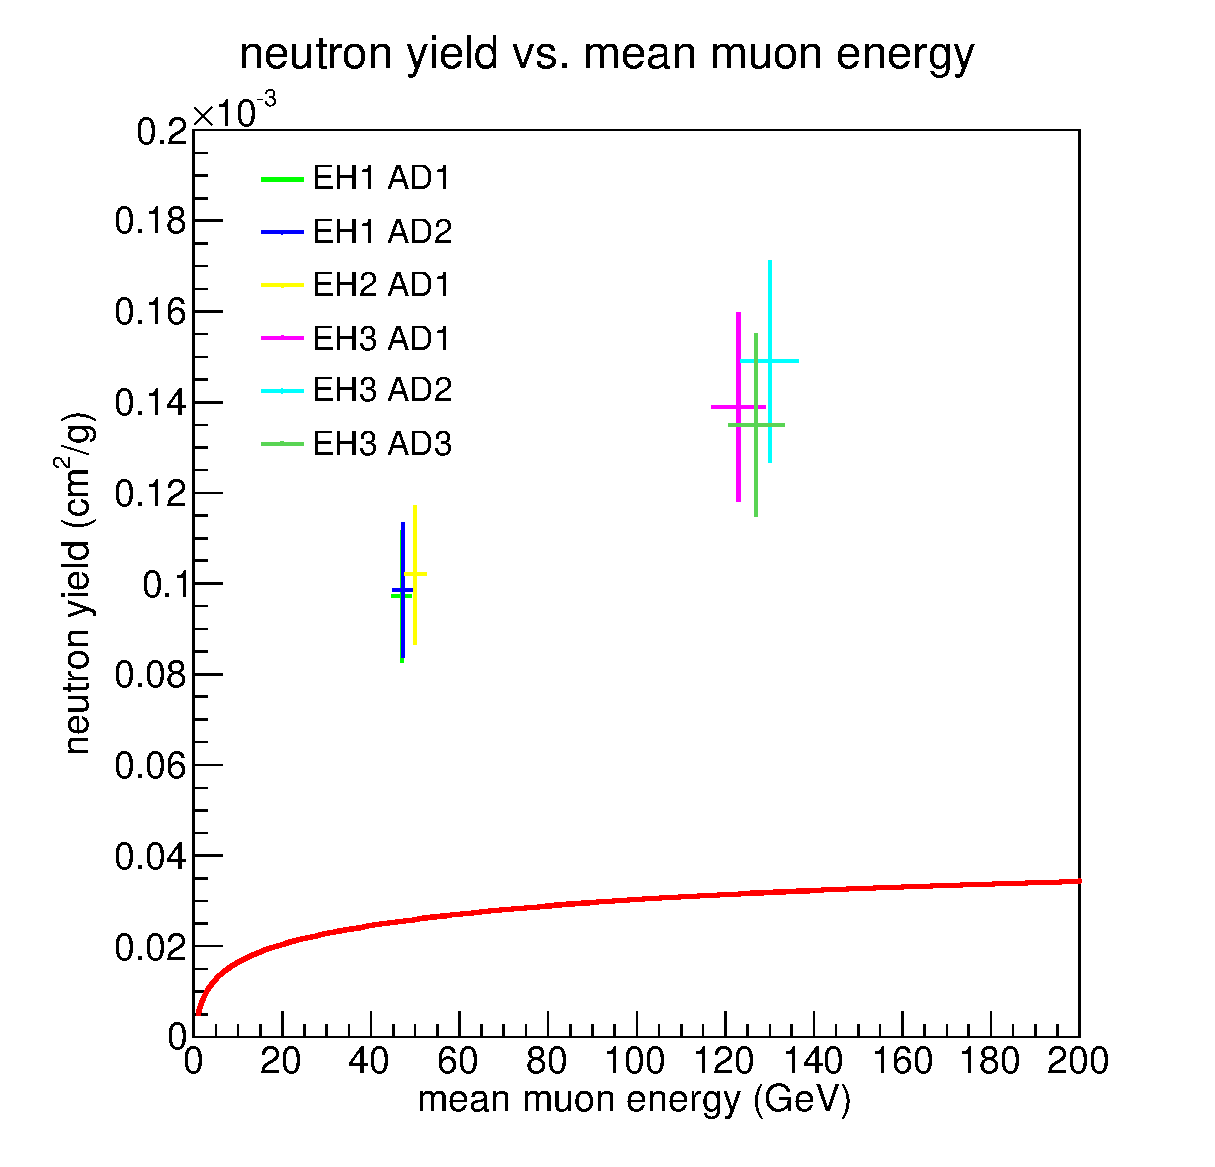
\includegraphics[width=.8\textwidth]{figures/chap7/yield_vs_energy_thesis.eps}
	\caption{Neutron yield as a function of the mean muon energy. The red curve is the calculated yield from the muon spallation process under the assumptions made in Chapter~\ref{chap:yield_theory}.}
	\label{fig:yield_vs_energy}
\end{figure}

Since muon trajectories are able to be reconstructed, the muon energy loss can be studied.
\begin{figure}
	\centering
	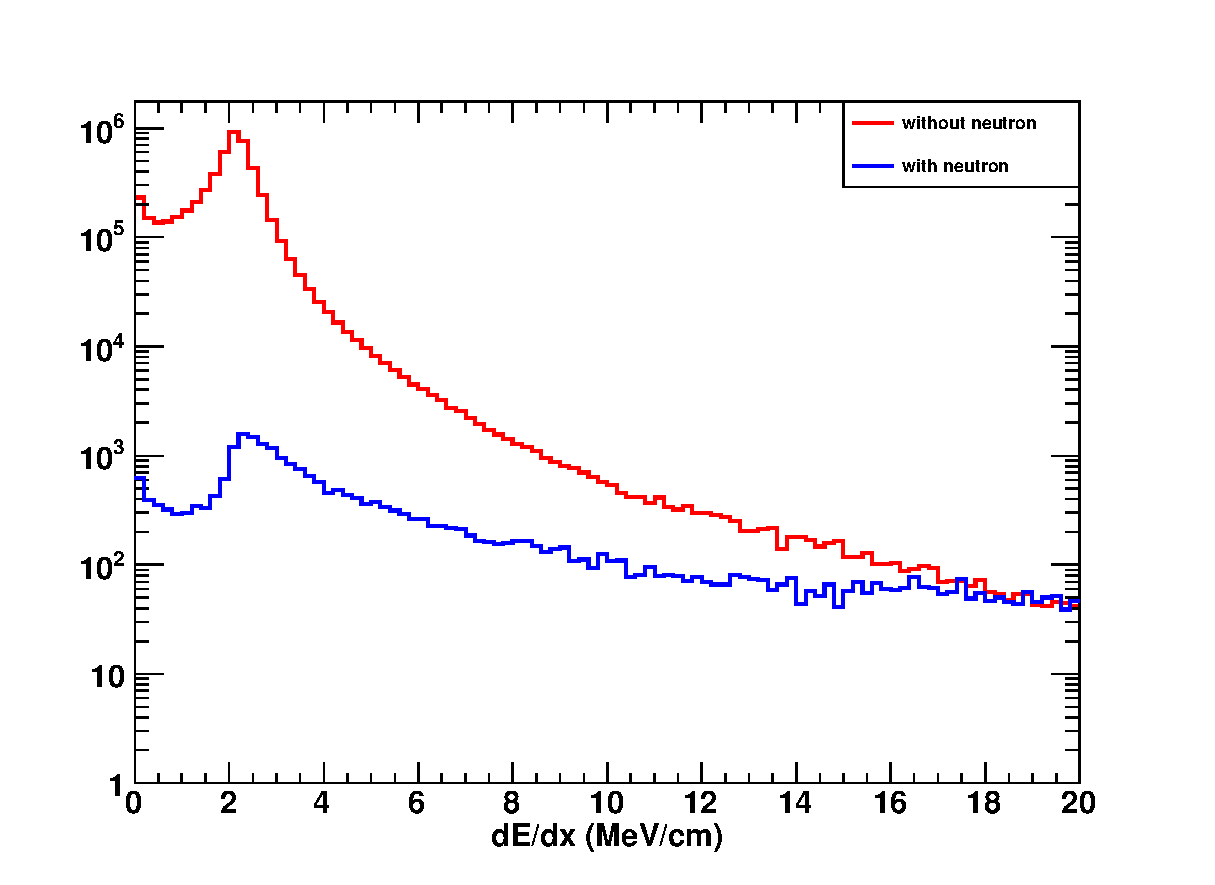
\includegraphics[width=.6\textwidth]{figures/chap7/dedx.eps}
	\caption{Muon energy loss for muons with and without induced neutrons.}
	\label{fig:dedx}
\end{figure}
Figure~\ref{fig:dedx} shows the muon energy loss in units of MeV/cm for muons with and without induced neutrons. The red histogram is the energy loss without associated neutrons and the blue one is the energy loss with associated neutrons. First we see both histograms peak at $\approx 2$ MeV/cm, corresponding to the minimum ionizing particles. However, the blue curve with-neutron histogram has a flatter tail, indicating extra energy deposition for muons with produced neutrons compared with those without produced neutrons.